\documentclass[11pt,a4paper]{report}	% report - article
\usepackage{graphicx}
\usepackage{fancyhdr} 
\usepackage{fancybox} 
\usepackage{psfrag}
\usepackage{boxedminipage} 
\usepackage{epsfig}
\usepackage{amsmath}
\usepackage[ngerman]{babel}
\usepackage[T1]{fontenc}	%fr Sonderzeichen s. latin1
\usepackage[latin1]{inputenc}   %fr Umlaute & scharfes s
\usepackage{times}
\usepackage{float}
\usepackage{amsmath,amssymb}
\usepackage[dvips, a4paper, raiselinks, breaklinks, colorlinks, bookmarks, bookmarksnumbered,citecolor = black, linkcolor = black]{hyperref}
\usepackage{zardozDipl} 
\usepackage{url}







%
%
%\fancypagestyle{plain}{%
%    \lhead{LaTeX - TeXnicCenter} %left head
%    \rhead{Vorlage V2.0} % right head
%    \lfoot{Institut fr Robotik}
%    \rfoot{\thepage}
%    \cfoot{}		%keine Seitenangabe zustzlich in der Mitte !!!
%    \renewcommand{\headrulewidth}{0.4pt}
%    \renewcommand{\footrulewidth}{0.4pt}
%}
%
\pagestyle{plain}
%
\pagenumbering{arabic}
%
%\newtheorem{Aufgabe}{Aufgabe}[section]
%\newtheorem{Hinweis}{Hinweis}[section]
%
%
%\renewcommand{\chaptermark}[1]{}%   %shows chapter left header
%     
\renewcommand{\sectionmark}[1]{\markright{\thesection\ #1}{}}
%
\newcommand{\qu}{\symbol{94}}  %"^" !!!
\newcommand{\MS}{MatLab/SimuLink }
%
%--------------------------------------------------
%
\setlength{\parindent}{0mm}




\setcounter{section}{0}

\begin{document}

		%\textwidth 16cm
%\textheight 25cm
%\topmargin 3.2cm
%\oddsidemargin 0mm
%\parindent 0pt

\thispagestyle{empty}

% Verschiebung der Coverpage in X und Y. Einheit in cm.
\def\DELTAX{0.8}
\def\DELTAY{4.0}


% -------- only change entries beginning here ----------------------------
%
% enter the title of the thesis
%
\def\title{Title of the thesis}
%
% choose type of work: 0 ... Dissertation
%                      1 ... Diplomarbeit
%                      2 ... Masterarbeit
\def\type{1}
%
%
% enter name of degree, see examples below
%
\def\degree{Diplomingenieur}
%\def\degree{Diplomingenieurin}
%\def\degree{Master of Science}
%\def\degree{Doktor}
%\def\degree{Doktorin}

% enter the study (Studienrichtung)
% e.g. Diplomstudium:
%\def\study{Technische Mathematik}
% e.g. Masterstudium:
% \def\study{Industriemathematik}
% e.g. Doktorratsstudium
%\def\study{Technischen Wissenschaften}
%\def\study{Naturwissenschaften}
\def\study{Mechatronik}


% enter the name of the student
%
\def\name{Max Mustermann}
%
%
% enter the name of the institute
% e.g.
% \def\institute{Institut f\"ur Industriemathematik}
%
\def\institute{Institut f\"ur Robotik}
%
%
% enter the name of the supervisor (who is also the first referee)
% was also the supervisor, do so by choosing the line with (Betreuung)
%
\def\firstreferee{o. Univ.--Prof.\ Dr.--Ing.\ habil.\ Hartmut\ Bremer}
%
%
% in case of a second referee: uncomment the following line and enter the name
%
%\def\secondreferee{Prof.\ Dr.--Ing.\ habil.\ Dr. h.c. i.R.\ Max \ Muster}
%
%
% if there has been assistance by further people uncomment the following line
% and enter the name(s). if there are several assistants speerate the names by \\
%
 \def\assist{Name of assistant}
%\def\assist{Name of first assistant \\ Name of second assistant}
%
%
% enter month year
\def\date{Juni, 2010}
%
%
% the vertival alignment heavily depends on the length of the title if there are
% one or two supervisors or referees. whereever indicated as a question
%      more space ???
% below you might add additional space via (several) \medskip or \bigskip.
% do not change anything else
% -------------------------------------------------------------------------------
%
\def\ifundefined#1{\expandafter\ifx\csname#1\endcsname\relax}
%
\unitlength 1cm
\definecolor{mygray}{gray}{.85}
\sffamily
\begin{picture}(0,0)(\DELTAX,\DELTAY)
\put(-2.6,5){\color{mygray}\rule{25cm}{2.6cm}}
\put(10.8,5.15){\small UNIVERSIT\"AT}
\put(13.62,5.15){\small LINZ}
\put(10.8,5.5){\small JOHANNES}
\put(13,5.5){\small KEPLER}
\put(15,5.15){\Huge JKU}
\put(14.75,5.15){\line(0,1){.6}}
\put(9.7,5.6){
\includegraphics[width=9mm]{wap_small}}
\put(0,1){
\includegraphics[width=3cm]{tnf}}
\put(3.2,1.4){\scriptsize Technisch-Naturwissenschaftliche}
\put(3.2,1.05){\scriptsize Fakult\"at}
\end{picture}
%
\vspace{\DELTAY cm}

\begin{center}
{\LARGE\bfseries\title}
\bigskip\bigskip\bigskip\par
{\Large\ifcase\type DISSERTATION\or DIPLOMARBEIT\or MASTERARBEIT\fi}
\bigskip\par
zur Erlangung des akademischen Grades
\bigskip\smallskip\par
{\Large\degree}
\bigskip\par
im \ifcase\type Doktoratsstudium der\or Diplomstudium\or Masterstudium\fi
\bigskip\smallskip\par
{\Large\study}
\end{center}
%
% more space ???
%\bigskip
\bigskip\bigskip\bigskip\par
Eingereicht von:
\smallskip\par
{\large\name}
\medskip\bigskip\par
Angefertigt am:
\smallskip\par
{\large\institute}
\medskip\bigskip\par
Beurteilung:
\smallskip\par
{\large\firstreferee}
\ifundefined{secondreferee}\else {\large (Betreuung)}
\smallskip\par
{\large\secondreferee}\fi
\ifundefined{assist}\else
\medskip\bigskip\par
Mitwirkung:
\smallskip\par
{\large\assist}
\fi
%
% more space ???
%\bigskip
\bigskip\bigskip\bigskip\par
{\large Linz, \date}

\rmfamily 
	

		\pagestyle{zardoz}
		
		\textheight 24cm
		\textwidth 16cm
		\oddsidemargin 8mm
		\topmargin -15mm
		\headheight 1cm
		\headsep 1cm


		\pagenumbering{roman}
		\setcounter{page}{1}
		\tableofcontents																																   

		%----------------------------------------------------------------------------------
		%										 L I S T  O F  F I G U R E S                                   
		%----------------------------------------------------------------------------------
%		\listoffigures																																		 
%		\addcontentsline{toc}{chapter}{List of Figures} 																	 

		%----------------------------------------------------------------------------------
		%										 L I S T  O F  T A B L E S                                     
		%----------------------------------------------------------------------------------
%		\listoftables																																		   
%		\addcontentsline{toc}{chapter}{List of Tables}																		 

		%----------------------------------------------------------------------------------
		%										 C H A P T E R S                                               
		%----------------------------------------------------------------------------------
		\pagebreak
		\pagenumbering{arabic}
    \setcounter{page}{1}																										
    	\chapter*{TODO}
		\begin{verbatim}
		* poner esquema de la placa de alimentacion del kinect, switch, conversor
		* tutorial to do a new model using google SketchUP
		* tutorial to make a new msgs and srv
		* explain the teleop_joy and teleop_key
		* explain the launch file
		* explain the server and client
		* make a diagram of all the system
		* make a class diagram
		* instalation driver canbus,
		* scan manual for the configuration of 424 to 232 converser
		* create a CD with all the code and models and documents
		* explicar AMCL -> http://www.ros.org/wiki/amcl
		* 
		\end{verbatim}    
    
    		\include{InstallROSinUbuntu}
		\include{InstallDevelopmentTools}
		\include{Downloadandcompilethestack}
		%\chapter{Install ROS in Ubuntu}

\section{Configure your Ubuntu repositories:}

Configure your Ubuntu repositories to allow {\bfseries restricted, universe, multiverse}. You can follow the Ubuntu guide ( https://help.ubuntu.com/community/Repositories/Ubuntu ) for instructions on doing this.

\section{Setup your sources.list:}


Setup your sources.list file to accept Debian packages from the ROS server.  
\newline

{\hspace{2em}\bfseries Ubuntu 9.04 (Jaunty)}

\hspace{4em}
sudo sh -c 'echo "deb http://code.ros.org/packages/ros/ubuntu jaunty main" > /etc/apt/sources.list.d/ros-latest.list'
\newline
 
{\hspace{2em}\bfseries Ubuntu 9.10 (Karmic)}

\hspace{4em}
sudo sh -c 'echo "deb http://code.ros.org/packages/ros/ubuntu karmic main" > /etc/apt/sources.list.d/ros-latest.list'
\newline

{\hspace{2em}\bfseries Ubuntu 10.04 (Lucid)}

\hspace{4em}
sudo sh -c 'echo "deb http://code.ros.org/packages/ros/ubuntu lucid main" > /etc/apt/sources.list.d/ros-latest.list'
\newline

{\hspace{2em}\bfseries Ubuntu 10.10 (Maverick)}

\hspace{4em}
sudo sh -c 'echo "deb http://code.ros.org/packages/ros/ubuntu maverick main" > /etc/apt/sources.list.d/ros-latest.list'
\newline

{\bfseries * (In this tutorial we will use the Ubuntu 10.10)}


\section{Set up your keys:}

\hspace{2em}wget http://code.ros.org/packages/ros.key -O - | sudo apt-key add -
\newline

\section{Installation}

Make sure you have re-indexed the ROS.org server:

    \hspace{2em} sudo apt-get update
\newline

Choose your preferred install:

{\hspace{2em}\bfseries ROS only:}

\hspace{4em}
sudo apt-get install ros-cturtle-ros
\newline


{\hspace{2em}\bfseries Base:} ROS plus robot-generic stacks (e.g. navigation, visualization)

\hspace{4em}
sudo apt-get install ros-cturtle-base
\newline


{\hspace{2em}\bfseries PR2:} ROS plus PR2-specific stacks, including PR2 simulator.

\hspace{4em}
sudo apt-get install ros-cturtle-pr2
\newline


{\hspace{2em}\bfseries PR2 All:} ROS plus PR2 and bleeding edge research/experimental stacks.

\hspace{4em}
sudo apt-get install ros-cturtle-pr2all
\newline

{\hspace{2em}\bfseries Stack-specific:} You can also install a specific ROS stack (replace underscores with dashes of the stack name):

\hspace{4em}
sudo apt-get install ros-cturtle-STACK

\hspace{4em}
sudo apt-get install ros-cturtle-slam-gmapping


\section{Environment setup}

It's convenient if the ROS environment variables are automatically added to your bash session every time a new shell is launched:
\newline

\hspace{2em} echo "source /opt/ros/cturtle/setup.bash" >> ~/.bashrc

\hspace{2em} . ~/.bashrc
\newline

If you just want to change the environment of your current shell, you can type:
\newline

\hspace{2em} source /opt/ros/cturtle/setup.bash
\newline

And with all this, the system must be installed.



		%\chapter{Download and install Code::Blocks}


		%\chapter{Install and configure git}
		%\chapter{Download repositories from AaronMR}
		%\chapter{Direction and velocity from the simulator}


		%\chapter{ROS tutorials}

\section{Launch simulator with navigation stack}

\begin{verbatim}

Setting up your robot using tf:
http://www.ros.org/wiki/navigation/Tutorials/RobotSetup/TF

urdf:
http://www.ros.org/wiki/urdf
http://www.ros.org/wiki/urdf/Tutorials/Create%20your%20own%20urdf%20file
http://www.ros.org/wiki/urdf/Tutorials/Create%20your%20own%20urdf%20file


:Stack Navigation
http://www.ros.org/wiki/navigation

Install kinect:
http://www.ros.org/wiki/kinect
http://www.ros.org/wiki/kinect/Tutorials/Getting%20Started
http://www.ros.org/wiki/kinect_calibration

gmapping:
http://www.ros.org/wiki/gmapping

Simulating the 2dnav Stack:
http://www.ros.org/wiki/pr2_2dnav_gazebo/Tutorials/Simulating the 2dnav Stack
\end{verbatim}

		%\chapter*{Building a Visual Robot Model with URDF from Scratch}

\begin{verbatim}
 Description: Learn how to build a visual model of a robot that you can view in Rviz

Keywords: URDF

Tutorial Level: BEGINNER

Next Tutorial: Making the Model Move, Adding Physical and Collision Properties to the Model, Cleaning up Models with Xacro

Tabla de Contenidos

   1. One Shape
   2. Multiple Shapes
   3. Origins
   4. Material Girl
   5. Finishing the Model

In this tutorial, we’re going to build a visual model of a robot that vaguely looks like R2D2. In later tutorials, you’ll learn how to articulate the model, add in some physical properties, generate neater code with xacro and make it move in Gazebo. But for now, we’re going to focus on getting the visual geometry correct.

In these tutorials, we’re going to rely on some tools and launch files from the urdf_tools package. All of the robot models mentioned in this tutorial can be found in the urdf_tutorial package.

One Shape

First, we’re just going to explore one simple shape. Here’s about as simple as a urdf as you can make. Source

[des]activar nros. de línea

   1 <?xml version="1.0"?>
   2 <robot name="myfirst">
   3   <link name="base_link">
   4     <visual>
   5       <geometry>
   6         <cylinder length="0.6" radius="0.2"/>
   7       </geometry>
   8     </visual>
   9   </link>
  10 </robot>

To translate the XML into English, this is a robot with the name myfirst, that contains only one link (a.k.a. part), whose visual component is just a cylinder .6 meters long with a .2 meter radius. This may seem like a lot of enclosing tags for a simple “hello world” type example, but it will get more complicated, trust me.

To examine the model, type roslaunch urdf_tutorial display.launch model:=01-myfirst.urdf This does three things. It

    * Loads the specified model into the parameter server
    *

      Runs nodes to publish the JointState and transforms (more on these later)
    * Starts Rviz with a configuration file 

This launch file assumes that 01-myfirst.urdf is in the same directory that you type the command in. Otherwise, you should say model:=$(find pkg-name)/01-myfirst.urdf where pkg-name is the name of the package that the file is in. All of the example files are in the urdf_tutorials package, so if you are in that package's directory, you can run the commands without modification.

The model we made should look like this

my first image

Things to note:

    * The fixed frame is transform frame where the center of the grid is located. Here, it’s a frame defined by our one link, base_link.
    * The visual element (the cylinder) has its origin at the center of its geometry as a default. Hence, half the cylinder is below the grid. 

Multiple Shapes

Now let’s look at how to add multiple shapes/links. If we just add more link elements to the urdf, the parser won’t know where to put them. So, we have to add joints. Joint elements can refer to both flexible and inflexible joints. We’ll start with inflexible, or fixed joints. Source

[des]activar nros. de línea

   1 <?xml version="1.0"?>
   2 <robot name="multipleshapes">
   3   <link name="base_link">
   4     <visual>
   5       <geometry>
   6         <cylinder length="0.6" radius="0.2"/>
   7       </geometry>
   8     </visual>
   9   </link>
  10 
  11   <link name="right_leg">
  12     <visual>
  13       <geometry>
  14         <box size="0.6 .2 .1"/>
  15       </geometry>
  16     </visual>
  17   </link>
  18 
  19   <joint name="base_to_right_leg" type="fixed">
  20     <parent link="base_link"/>
  21     <child link="right_leg"/>
  22   </joint>
  23 
  24 </robot>

    * Note how we defined a 0.6m x 0.2m x 0.1m box
    * The joint is defined in terms of a parent and a child. URDF is ultimately a tree structure with one root link. This means that the leg’s position in dependent on the base_link’s position. 

roslaunch urdf_tutorial display.launch model:=02-multipleshapes.urdf Multiple Shapes

Both of the shapes overlap with each other, because they share the same origin. If we want them not to overlap we must define more origins.

Origins

So R2D2’s leg attaches to the top half of his torso, on the side. So that’s where we specify the origin of the JOINT to be. Also, it doesn’t attach to the middle of the leg, it attaches to the upper part, so we must offset the origin for the leg as well. We also rotate the leg so it is upright. Source

[des]activar nros. de línea

   1 <?xml version="1.0"?>
   2 <robot name="origins">
   3   <link name="base_link">
   4     <visual>
   5       <geometry>
   6         <cylinder length="0.6" radius="0.2"/>
   7       </geometry>
   8     </visual>
   9   </link>
  10 
  11   <link name="right_leg">
  12     <visual>
  13       <geometry>
  14         <box size="0.6 .2 .1"/>
  15       </geometry>
  16       <origin rpy="0 1.57075 0" xyz="0 0 -0.3"/>
  17     </visual>
  18   </link>
  19 
  20   <joint name="base_to_right_leg" type="fixed">
  21     <parent link="base_link"/>
  22     <child link="right_leg"/>
  23     <origin xyz="0.22 0 .25"/>
  24   </joint>
  25 
  26 </robot>

    * Let’s start by examining the joint’s origin. It is defined in terms of the parent’s reference frame. So we are .21 meters in the x direction (left) and .25 meters in the z direction (up). This means that the origin for the child link will be up and to the left, regardless of the child link’s visual origin tag. Since we didn’t specify a rpy (roll pitch yaw) attribute, the child frame will be default have the same orientation as the parent frame.
    * Now, looking at the leg’s visual origin, it has both a xyz and rpy offset. This defines where the center of the visual element should be, relative to its origin. Since we want the leg to attach at the top, we offset the origin down by setting the z offset to be -.4 meters. And since we want the long part of the leg to be parallel to the z axis, we rotate the visual part PI/2 around the Y axis. 

roslaunch urdf_tutorial display.launch model:=03-origins.urdf Origins Screenshot

    * The launch file runs packages that will create TF frames for each link in your model based on your URDF. Rviz uses this information to figure out where to display each shape.
    * If a TF frame does not exist for a given URDF link, then it will be placed at the origin in white. 

Material Girl

“Alright,” I hear you say. “That’s very cute, but not everyone owns a B21. My robot and R2D2 are not red!” That’s a good point. Let’s take a look at the material tag. Source

[des]activar nros. de línea

   1 <?xml version="1.0"?>
   2 <robot name="materials">
   3   <link name="base_link">
   4     <visual>
   5       <geometry>
   6         <cylinder length="0.6" radius="0.2"/>
   7       </geometry>
   8       <material name="blue">
   9         <color rgba="0 0 .8 1"/>
  10       </material>
  11     </visual>
  12   </link>
  13 
  14   <link name="right_leg">
  15     <visual>
  16       <geometry>
  17         <box size="0.6 .2 .1"/>
  18       </geometry>
  19       <origin rpy="0 1.57075 0" xyz="0 0 -0.3"/>
  20       <material name="white">
  21         <color rgba="1 1 1 1"/>
  22       </material>
  23     </visual>
  24   </link>
  25 
  26   <joint name="base_to_right_leg" type="fixed">
  27     <parent link="base_link"/>
  28     <child link="right_leg"/>
  29     <origin xyz="0.22 0 .25"/>
  30   </joint>
  31 
  32   <link name="left_leg">
  33     <visual>
  34       <geometry>
  35         <box size="0.6 .2 .1"/>
  36       </geometry>
  37       <origin rpy="0 1.57075 0" xyz="0 0 -0.3"/>
  38       <material name="white"/>
  39     </visual>
  40   </link>
  41 
  42   <joint name="base_to_left_leg" type="fixed">
  43     <parent link="base_link"/>
  44     <child link="left_leg"/>
  45     <origin xyz="-0.22 0 .25"/>
  46   </joint>
  47 
  48 </robot>

    * The body is now blue. By adding the first material tag, we’ve defined a new material called “blue”, with the red, green, blue and alpha channels defined as 0,0,.8 and 1 respectively. All of the values can be in the range [0,1].
    * The white material is defined similarly
    * For the second leg, we can refer to the material just by name, since it’s been previously defined. No one will complain if you redefine it though.
    * You can also use a texture to specify an image file to be used for coloring the object 

roslaunch urdf_tutorial display.launch model:=04-materials.urdf Materials Screenshot

Finishing the Model

Now we finish the model off with a few more shapes. Most notably, we add a sphere and a some meshes. We’ll also add few other pieces that we’ll use later. Source

roslaunch urdf_tutorial display.launch model:=05-visual.urdf Visual Screenshot

How to add the sphere should be fairly self explanatory
[des]activar nros. de línea

   1   <link name="head">
   2     <visual>
   3       <geometry>
   4         <sphere radius="0.2"/>
   5       </geometry>
   6       <material name="white"/>
   7     </visual>
   8   </link>

The meshes here were borrowed from the PR2, meaning you’ll need the package pr2_description to be able to see them.
[des]activar nros. de línea

   1   <link name="left_gripper">
   2     <visual>
   3       <geometry>
   4         <mesh filename="package://pr2_description/meshes/gripper_v0/l_finger.dae"/>
   5       </geometry>
   6     </visual>
   7   </link>

    * The meshes can be imported in a number of different formats. STL is fairly common, but the engine also supports DAE, which can have its own color data, meaning you don’t have to specify the color data.
    * Meshes can also be sized using relative scaling parameters or a bounding box size. 

There you have it. A R2D2-like URDF model. Now you can continue on to the next step, making it move. 
\end{verbatim}


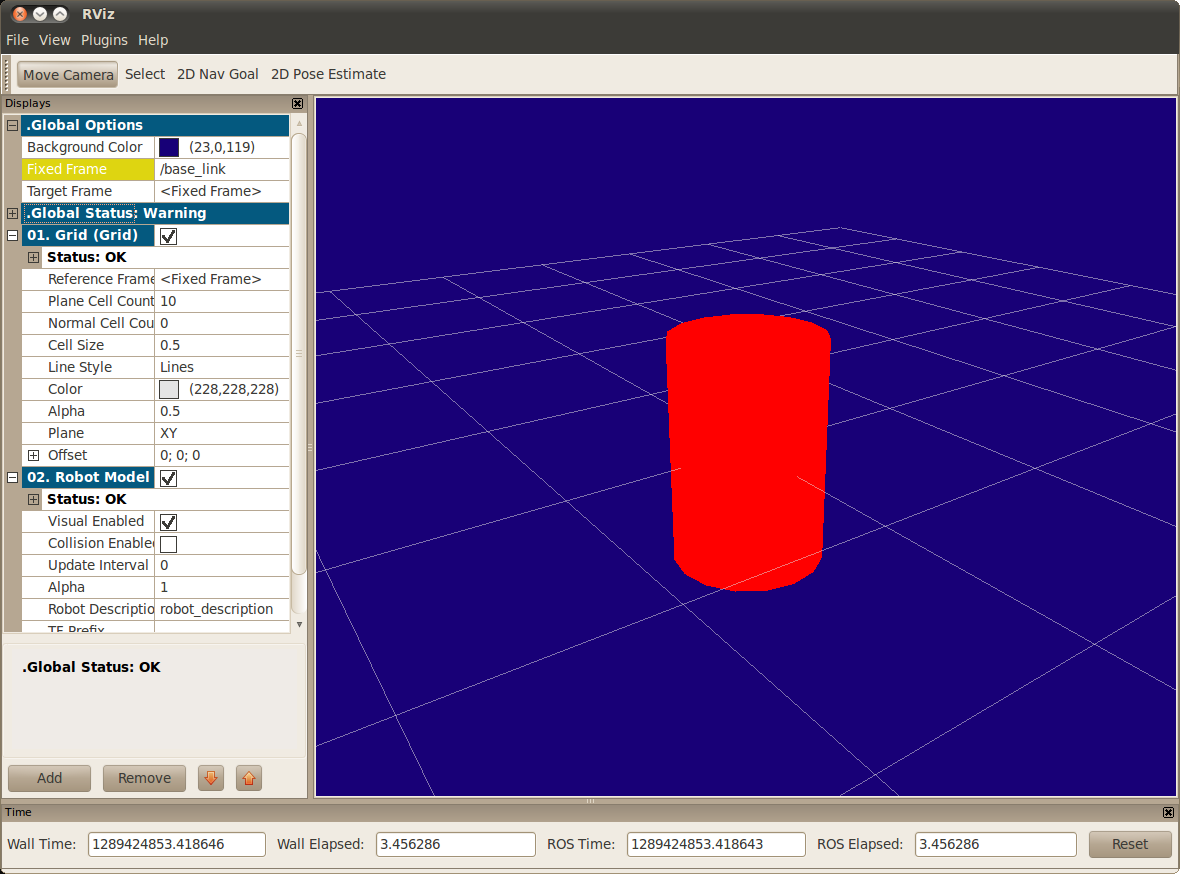
\includegraphics[width=0.5\textwidth,angle=0]{tutorials/tutorial_2/img/myfirst.png}	

		%\chapter*{Building a Visual Robot Model with URDF from Scratch}

\begin{verbatim}
 Description: Learn how to build a visual model of a robot that you can view in Rviz

Keywords: URDF

Tutorial Level: BEGINNER

Next Tutorial: Making the Model Move, Adding Physical and Collision Properties to the Model, Cleaning up Models with Xacro

Tabla de Contenidos

   1. One Shape
   2. Multiple Shapes
   3. Origins
   4. Material Girl
   5. Finishing the Model

In this tutorial, we’re going to build a visual model of a robot that vaguely looks like R2D2. In later tutorials, you’ll learn how to articulate the model, add in some physical properties, generate neater code with xacro and make it move in Gazebo. But for now, we’re going to focus on getting the visual geometry correct.

In these tutorials, we’re going to rely on some tools and launch files from the urdf_tools package. All of the robot models mentioned in this tutorial can be found in the urdf_tutorial package.

One Shape

First, we’re just going to explore one simple shape. Here’s about as simple as a urdf as you can make. Source

[des]activar nros. de línea

   1 <?xml version="1.0"?>
   2 <robot name="myfirst">
   3   <link name="base_link">
   4     <visual>
   5       <geometry>
   6         <cylinder length="0.6" radius="0.2"/>
   7       </geometry>
   8     </visual>
   9   </link>
  10 </robot>

To translate the XML into English, this is a robot with the name myfirst, that contains only one link (a.k.a. part), whose visual component is just a cylinder .6 meters long with a .2 meter radius. This may seem like a lot of enclosing tags for a simple “hello world” type example, but it will get more complicated, trust me.

To examine the model, type roslaunch urdf_tutorial display.launch model:=01-myfirst.urdf This does three things. It

    * Loads the specified model into the parameter server
    *

      Runs nodes to publish the JointState and transforms (more on these later)
    * Starts Rviz with a configuration file 

This launch file assumes that 01-myfirst.urdf is in the same directory that you type the command in. Otherwise, you should say model:=$(find pkg-name)/01-myfirst.urdf where pkg-name is the name of the package that the file is in. All of the example files are in the urdf_tutorials package, so if you are in that package's directory, you can run the commands without modification.

The model we made should look like this

my first image

Things to note:

    * The fixed frame is transform frame where the center of the grid is located. Here, it’s a frame defined by our one link, base_link.
    * The visual element (the cylinder) has its origin at the center of its geometry as a default. Hence, half the cylinder is below the grid. 

Multiple Shapes

Now let’s look at how to add multiple shapes/links. If we just add more link elements to the urdf, the parser won’t know where to put them. So, we have to add joints. Joint elements can refer to both flexible and inflexible joints. We’ll start with inflexible, or fixed joints. Source

[des]activar nros. de línea

   1 <?xml version="1.0"?>
   2 <robot name="multipleshapes">
   3   <link name="base_link">
   4     <visual>
   5       <geometry>
   6         <cylinder length="0.6" radius="0.2"/>
   7       </geometry>
   8     </visual>
   9   </link>
  10 
  11   <link name="right_leg">
  12     <visual>
  13       <geometry>
  14         <box size="0.6 .2 .1"/>
  15       </geometry>
  16     </visual>
  17   </link>
  18 
  19   <joint name="base_to_right_leg" type="fixed">
  20     <parent link="base_link"/>
  21     <child link="right_leg"/>
  22   </joint>
  23 
  24 </robot>

    * Note how we defined a 0.6m x 0.2m x 0.1m box
    * The joint is defined in terms of a parent and a child. URDF is ultimately a tree structure with one root link. This means that the leg’s position in dependent on the base_link’s position. 

roslaunch urdf_tutorial display.launch model:=02-multipleshapes.urdf Multiple Shapes

Both of the shapes overlap with each other, because they share the same origin. If we want them not to overlap we must define more origins.

Origins

So R2D2’s leg attaches to the top half of his torso, on the side. So that’s where we specify the origin of the JOINT to be. Also, it doesn’t attach to the middle of the leg, it attaches to the upper part, so we must offset the origin for the leg as well. We also rotate the leg so it is upright. Source

[des]activar nros. de línea

   1 <?xml version="1.0"?>
   2 <robot name="origins">
   3   <link name="base_link">
   4     <visual>
   5       <geometry>
   6         <cylinder length="0.6" radius="0.2"/>
   7       </geometry>
   8     </visual>
   9   </link>
  10 
  11   <link name="right_leg">
  12     <visual>
  13       <geometry>
  14         <box size="0.6 .2 .1"/>
  15       </geometry>
  16       <origin rpy="0 1.57075 0" xyz="0 0 -0.3"/>
  17     </visual>
  18   </link>
  19 
  20   <joint name="base_to_right_leg" type="fixed">
  21     <parent link="base_link"/>
  22     <child link="right_leg"/>
  23     <origin xyz="0.22 0 .25"/>
  24   </joint>
  25 
  26 </robot>

    * Let’s start by examining the joint’s origin. It is defined in terms of the parent’s reference frame. So we are .21 meters in the x direction (left) and .25 meters in the z direction (up). This means that the origin for the child link will be up and to the left, regardless of the child link’s visual origin tag. Since we didn’t specify a rpy (roll pitch yaw) attribute, the child frame will be default have the same orientation as the parent frame.
    * Now, looking at the leg’s visual origin, it has both a xyz and rpy offset. This defines where the center of the visual element should be, relative to its origin. Since we want the leg to attach at the top, we offset the origin down by setting the z offset to be -.4 meters. And since we want the long part of the leg to be parallel to the z axis, we rotate the visual part PI/2 around the Y axis. 

roslaunch urdf_tutorial display.launch model:=03-origins.urdf Origins Screenshot

    * The launch file runs packages that will create TF frames for each link in your model based on your URDF. Rviz uses this information to figure out where to display each shape.
    * If a TF frame does not exist for a given URDF link, then it will be placed at the origin in white. 

Material Girl

“Alright,” I hear you say. “That’s very cute, but not everyone owns a B21. My robot and R2D2 are not red!” That’s a good point. Let’s take a look at the material tag. Source

[des]activar nros. de línea

   1 <?xml version="1.0"?>
   2 <robot name="materials">
   3   <link name="base_link">
   4     <visual>
   5       <geometry>
   6         <cylinder length="0.6" radius="0.2"/>
   7       </geometry>
   8       <material name="blue">
   9         <color rgba="0 0 .8 1"/>
  10       </material>
  11     </visual>
  12   </link>
  13 
  14   <link name="right_leg">
  15     <visual>
  16       <geometry>
  17         <box size="0.6 .2 .1"/>
  18       </geometry>
  19       <origin rpy="0 1.57075 0" xyz="0 0 -0.3"/>
  20       <material name="white">
  21         <color rgba="1 1 1 1"/>
  22       </material>
  23     </visual>
  24   </link>
  25 
  26   <joint name="base_to_right_leg" type="fixed">
  27     <parent link="base_link"/>
  28     <child link="right_leg"/>
  29     <origin xyz="0.22 0 .25"/>
  30   </joint>
  31 
  32   <link name="left_leg">
  33     <visual>
  34       <geometry>
  35         <box size="0.6 .2 .1"/>
  36       </geometry>
  37       <origin rpy="0 1.57075 0" xyz="0 0 -0.3"/>
  38       <material name="white"/>
  39     </visual>
  40   </link>
  41 
  42   <joint name="base_to_left_leg" type="fixed">
  43     <parent link="base_link"/>
  44     <child link="left_leg"/>
  45     <origin xyz="-0.22 0 .25"/>
  46   </joint>
  47 
  48 </robot>

    * The body is now blue. By adding the first material tag, we’ve defined a new material called “blue”, with the red, green, blue and alpha channels defined as 0,0,.8 and 1 respectively. All of the values can be in the range [0,1].
    * The white material is defined similarly
    * For the second leg, we can refer to the material just by name, since it’s been previously defined. No one will complain if you redefine it though.
    * You can also use a texture to specify an image file to be used for coloring the object 

roslaunch urdf_tutorial display.launch model:=04-materials.urdf Materials Screenshot

Finishing the Model

Now we finish the model off with a few more shapes. Most notably, we add a sphere and a some meshes. We’ll also add few other pieces that we’ll use later. Source

roslaunch urdf_tutorial display.launch model:=05-visual.urdf Visual Screenshot

How to add the sphere should be fairly self explanatory
[des]activar nros. de línea

   1   <link name="head">
   2     <visual>
   3       <geometry>
   4         <sphere radius="0.2"/>
   5       </geometry>
   6       <material name="white"/>
   7     </visual>
   8   </link>

The meshes here were borrowed from the PR2, meaning you’ll need the package pr2_description to be able to see them.
[des]activar nros. de línea

   1   <link name="left_gripper">
   2     <visual>
   3       <geometry>
   4         <mesh filename="package://pr2_description/meshes/gripper_v0/l_finger.dae"/>
   5       </geometry>
   6     </visual>
   7   </link>

    * The meshes can be imported in a number of different formats. STL is fairly common, but the engine also supports DAE, which can have its own color data, meaning you don’t have to specify the color data.
    * Meshes can also be sized using relative scaling parameters or a bounding box size. 

There you have it. A R2D2-like URDF model. Now you can continue on to the next step, making it move. 
\end{verbatim}


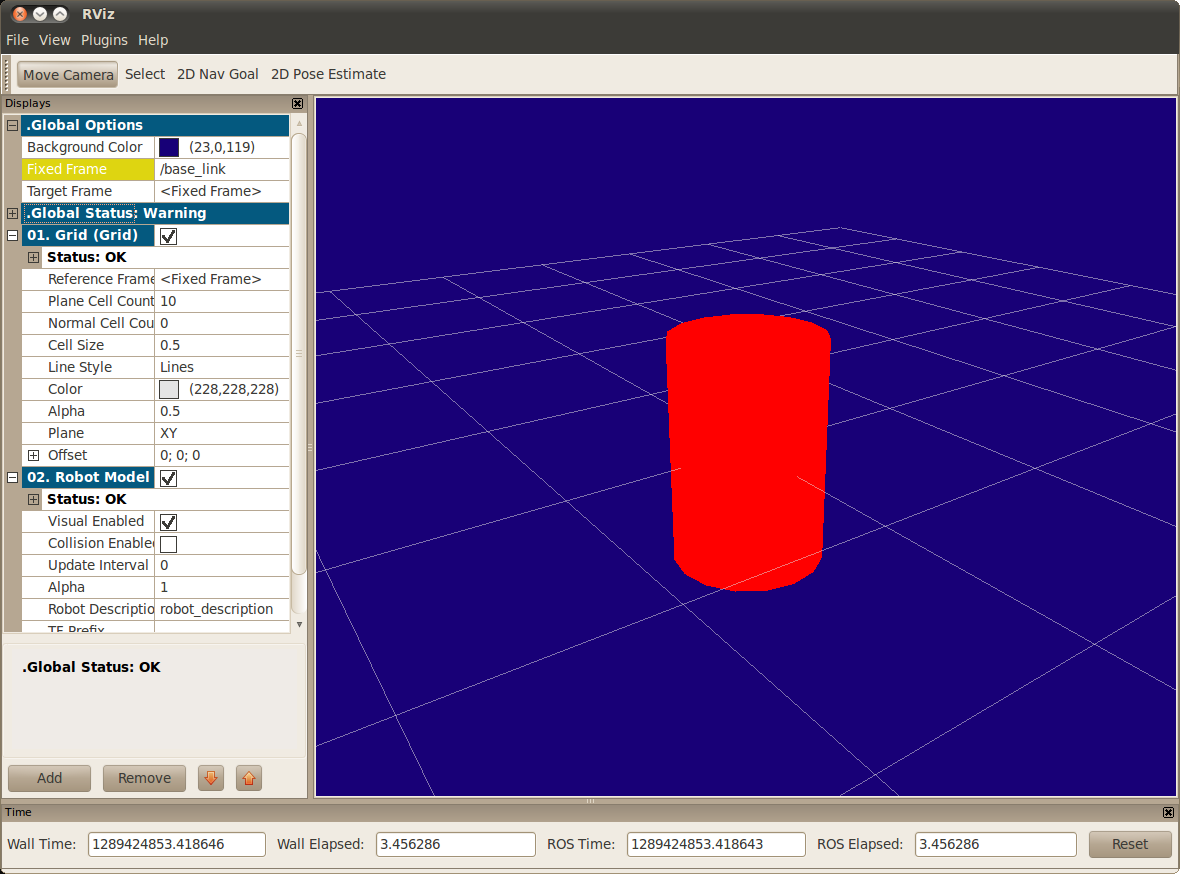
\includegraphics[width=0.5\textwidth,angle=0]{tutorials/tutorial_2/img/myfirst.png}	

		%\include{Navigation}
		%\chapter*{Building a Visual Robot Model with URDF from Scratch}

\begin{verbatim}
 Description: Learn how to build a visual model of a robot that you can view in Rviz

Keywords: URDF

Tutorial Level: BEGINNER

Next Tutorial: Making the Model Move, Adding Physical and Collision Properties to the Model, Cleaning up Models with Xacro

Tabla de Contenidos

   1. One Shape
   2. Multiple Shapes
   3. Origins
   4. Material Girl
   5. Finishing the Model

In this tutorial, we’re going to build a visual model of a robot that vaguely looks like R2D2. In later tutorials, you’ll learn how to articulate the model, add in some physical properties, generate neater code with xacro and make it move in Gazebo. But for now, we’re going to focus on getting the visual geometry correct.

In these tutorials, we’re going to rely on some tools and launch files from the urdf_tools package. All of the robot models mentioned in this tutorial can be found in the urdf_tutorial package.

One Shape

First, we’re just going to explore one simple shape. Here’s about as simple as a urdf as you can make. Source

[des]activar nros. de línea

   1 <?xml version="1.0"?>
   2 <robot name="myfirst">
   3   <link name="base_link">
   4     <visual>
   5       <geometry>
   6         <cylinder length="0.6" radius="0.2"/>
   7       </geometry>
   8     </visual>
   9   </link>
  10 </robot>

To translate the XML into English, this is a robot with the name myfirst, that contains only one link (a.k.a. part), whose visual component is just a cylinder .6 meters long with a .2 meter radius. This may seem like a lot of enclosing tags for a simple “hello world” type example, but it will get more complicated, trust me.

To examine the model, type roslaunch urdf_tutorial display.launch model:=01-myfirst.urdf This does three things. It

    * Loads the specified model into the parameter server
    *

      Runs nodes to publish the JointState and transforms (more on these later)
    * Starts Rviz with a configuration file 

This launch file assumes that 01-myfirst.urdf is in the same directory that you type the command in. Otherwise, you should say model:=$(find pkg-name)/01-myfirst.urdf where pkg-name is the name of the package that the file is in. All of the example files are in the urdf_tutorials package, so if you are in that package's directory, you can run the commands without modification.

The model we made should look like this

my first image

Things to note:

    * The fixed frame is transform frame where the center of the grid is located. Here, it’s a frame defined by our one link, base_link.
    * The visual element (the cylinder) has its origin at the center of its geometry as a default. Hence, half the cylinder is below the grid. 

Multiple Shapes

Now let’s look at how to add multiple shapes/links. If we just add more link elements to the urdf, the parser won’t know where to put them. So, we have to add joints. Joint elements can refer to both flexible and inflexible joints. We’ll start with inflexible, or fixed joints. Source

[des]activar nros. de línea

   1 <?xml version="1.0"?>
   2 <robot name="multipleshapes">
   3   <link name="base_link">
   4     <visual>
   5       <geometry>
   6         <cylinder length="0.6" radius="0.2"/>
   7       </geometry>
   8     </visual>
   9   </link>
  10 
  11   <link name="right_leg">
  12     <visual>
  13       <geometry>
  14         <box size="0.6 .2 .1"/>
  15       </geometry>
  16     </visual>
  17   </link>
  18 
  19   <joint name="base_to_right_leg" type="fixed">
  20     <parent link="base_link"/>
  21     <child link="right_leg"/>
  22   </joint>
  23 
  24 </robot>

    * Note how we defined a 0.6m x 0.2m x 0.1m box
    * The joint is defined in terms of a parent and a child. URDF is ultimately a tree structure with one root link. This means that the leg’s position in dependent on the base_link’s position. 

roslaunch urdf_tutorial display.launch model:=02-multipleshapes.urdf Multiple Shapes

Both of the shapes overlap with each other, because they share the same origin. If we want them not to overlap we must define more origins.

Origins

So R2D2’s leg attaches to the top half of his torso, on the side. So that’s where we specify the origin of the JOINT to be. Also, it doesn’t attach to the middle of the leg, it attaches to the upper part, so we must offset the origin for the leg as well. We also rotate the leg so it is upright. Source

[des]activar nros. de línea

   1 <?xml version="1.0"?>
   2 <robot name="origins">
   3   <link name="base_link">
   4     <visual>
   5       <geometry>
   6         <cylinder length="0.6" radius="0.2"/>
   7       </geometry>
   8     </visual>
   9   </link>
  10 
  11   <link name="right_leg">
  12     <visual>
  13       <geometry>
  14         <box size="0.6 .2 .1"/>
  15       </geometry>
  16       <origin rpy="0 1.57075 0" xyz="0 0 -0.3"/>
  17     </visual>
  18   </link>
  19 
  20   <joint name="base_to_right_leg" type="fixed">
  21     <parent link="base_link"/>
  22     <child link="right_leg"/>
  23     <origin xyz="0.22 0 .25"/>
  24   </joint>
  25 
  26 </robot>

    * Let’s start by examining the joint’s origin. It is defined in terms of the parent’s reference frame. So we are .21 meters in the x direction (left) and .25 meters in the z direction (up). This means that the origin for the child link will be up and to the left, regardless of the child link’s visual origin tag. Since we didn’t specify a rpy (roll pitch yaw) attribute, the child frame will be default have the same orientation as the parent frame.
    * Now, looking at the leg’s visual origin, it has both a xyz and rpy offset. This defines where the center of the visual element should be, relative to its origin. Since we want the leg to attach at the top, we offset the origin down by setting the z offset to be -.4 meters. And since we want the long part of the leg to be parallel to the z axis, we rotate the visual part PI/2 around the Y axis. 

roslaunch urdf_tutorial display.launch model:=03-origins.urdf Origins Screenshot

    * The launch file runs packages that will create TF frames for each link in your model based on your URDF. Rviz uses this information to figure out where to display each shape.
    * If a TF frame does not exist for a given URDF link, then it will be placed at the origin in white. 

Material Girl

“Alright,” I hear you say. “That’s very cute, but not everyone owns a B21. My robot and R2D2 are not red!” That’s a good point. Let’s take a look at the material tag. Source

[des]activar nros. de línea

   1 <?xml version="1.0"?>
   2 <robot name="materials">
   3   <link name="base_link">
   4     <visual>
   5       <geometry>
   6         <cylinder length="0.6" radius="0.2"/>
   7       </geometry>
   8       <material name="blue">
   9         <color rgba="0 0 .8 1"/>
  10       </material>
  11     </visual>
  12   </link>
  13 
  14   <link name="right_leg">
  15     <visual>
  16       <geometry>
  17         <box size="0.6 .2 .1"/>
  18       </geometry>
  19       <origin rpy="0 1.57075 0" xyz="0 0 -0.3"/>
  20       <material name="white">
  21         <color rgba="1 1 1 1"/>
  22       </material>
  23     </visual>
  24   </link>
  25 
  26   <joint name="base_to_right_leg" type="fixed">
  27     <parent link="base_link"/>
  28     <child link="right_leg"/>
  29     <origin xyz="0.22 0 .25"/>
  30   </joint>
  31 
  32   <link name="left_leg">
  33     <visual>
  34       <geometry>
  35         <box size="0.6 .2 .1"/>
  36       </geometry>
  37       <origin rpy="0 1.57075 0" xyz="0 0 -0.3"/>
  38       <material name="white"/>
  39     </visual>
  40   </link>
  41 
  42   <joint name="base_to_left_leg" type="fixed">
  43     <parent link="base_link"/>
  44     <child link="left_leg"/>
  45     <origin xyz="-0.22 0 .25"/>
  46   </joint>
  47 
  48 </robot>

    * The body is now blue. By adding the first material tag, we’ve defined a new material called “blue”, with the red, green, blue and alpha channels defined as 0,0,.8 and 1 respectively. All of the values can be in the range [0,1].
    * The white material is defined similarly
    * For the second leg, we can refer to the material just by name, since it’s been previously defined. No one will complain if you redefine it though.
    * You can also use a texture to specify an image file to be used for coloring the object 

roslaunch urdf_tutorial display.launch model:=04-materials.urdf Materials Screenshot

Finishing the Model

Now we finish the model off with a few more shapes. Most notably, we add a sphere and a some meshes. We’ll also add few other pieces that we’ll use later. Source

roslaunch urdf_tutorial display.launch model:=05-visual.urdf Visual Screenshot

How to add the sphere should be fairly self explanatory
[des]activar nros. de línea

   1   <link name="head">
   2     <visual>
   3       <geometry>
   4         <sphere radius="0.2"/>
   5       </geometry>
   6       <material name="white"/>
   7     </visual>
   8   </link>

The meshes here were borrowed from the PR2, meaning you’ll need the package pr2_description to be able to see them.
[des]activar nros. de línea

   1   <link name="left_gripper">
   2     <visual>
   3       <geometry>
   4         <mesh filename="package://pr2_description/meshes/gripper_v0/l_finger.dae"/>
   5       </geometry>
   6     </visual>
   7   </link>

    * The meshes can be imported in a number of different formats. STL is fairly common, but the engine also supports DAE, which can have its own color data, meaning you don’t have to specify the color data.
    * Meshes can also be sized using relative scaling parameters or a bounding box size. 

There you have it. A R2D2-like URDF model. Now you can continue on to the next step, making it move. 
\end{verbatim}


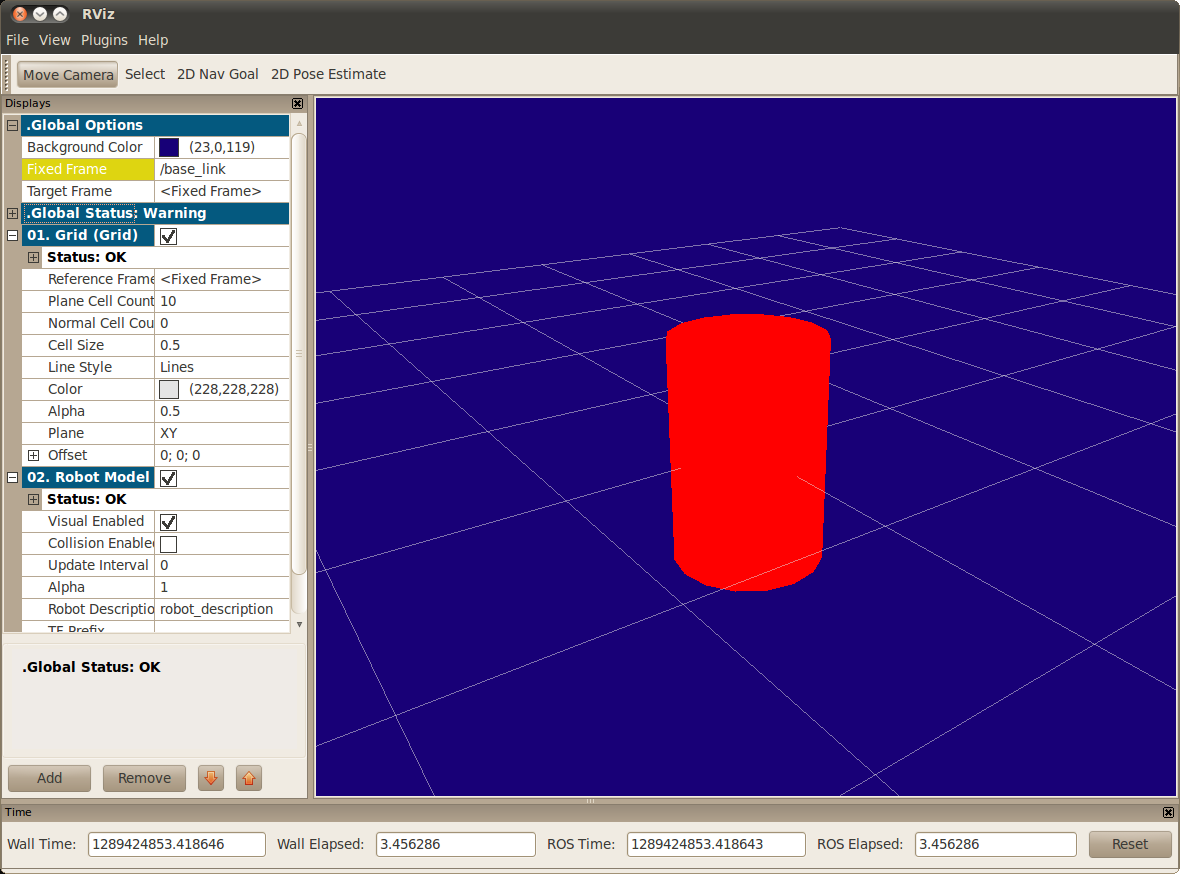
\includegraphics[width=0.5\textwidth,angle=0]{tutorials/tutorial_2/img/myfirst.png}	



\end{document}
